\subsection{Conics}\label{sec:Conics}

In this section we review equations of parabolas, circles, ellipses and hyperbolas.
We will give the equations of various conics in \dfont{standard form} along with a sketch.
A useful mnemonic is the following.\\

\begin{formulabox}[Mnemonic]
In each conic formula presented, the terms `$x-h$' and `$y-k$' will always appear. 
The point $(h,k)$ will alway represent either the centre or vertex of the particular conic.
\end{formulabox}

%%%%%%%%%%%%%%%%%%%%%%%%%%%%%%%%%%%%%%%%%%%%%%%%%%%%%%%%%%%
%\subsubsection{Parabolas, circles, ellipses and hyperbolas}

\bigskip\noindent
\dfont{Vertical Parabola:} The equation of a vertical parabola is:
$$y-k=a(x-h)^2$$
$$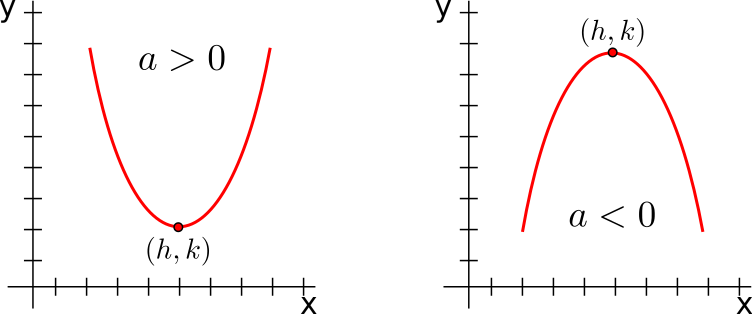
\includegraphics[width=85mm]{images/conics1}$$
\begin{multicols}{2}
\begin{itemize}
	\item $(h,k)$ is the \ifont{vertex} of the parabola.
	\item $a$ is the vertical \ifont{stretch factor}. 
	\item If $a>0$, the parabola opens \ifont{upward}.
	\item If $a<0$, the parabola opens \ifont{downward}.
\end{itemize}
\end{multicols}

\bigskip\noindent
\dfont{Horizontal Parabola:} The equation of a horizontal parabola is:
$$x-h=a(y-k)^2$$
$$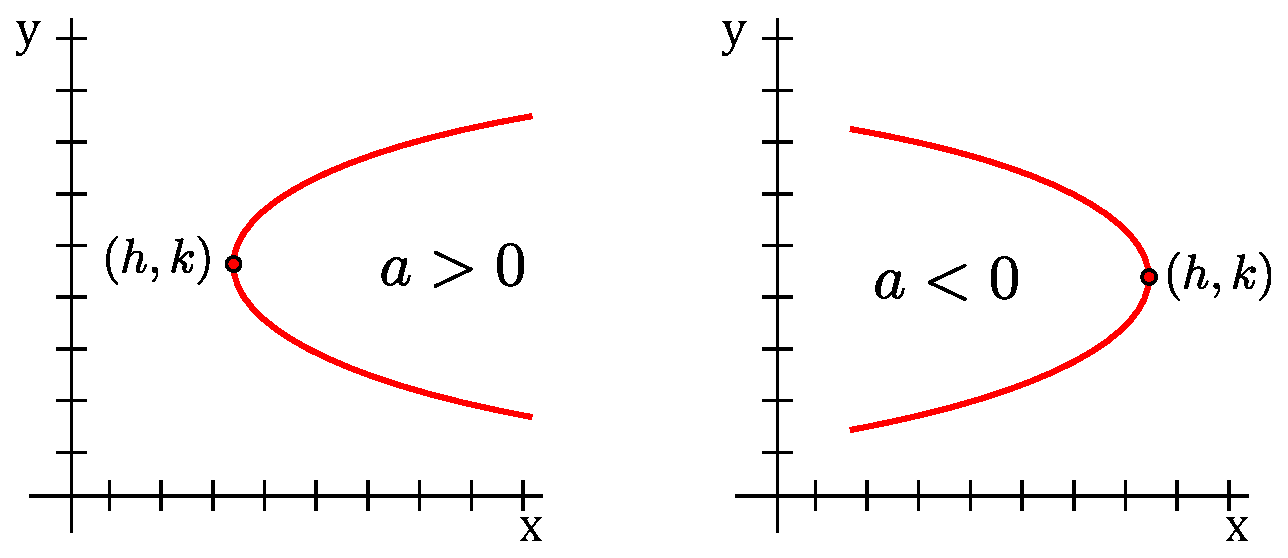
\includegraphics[width=85mm]{images/conics2}$$
\begin{multicols}{2}
\begin{itemize}
	\item $(h,k)$ is the \ifont{vertex} of the parabola.
	\item $a$ is the horizontal \ifont{stretch factor}. 
	\item If $a>0$, the parabola opens \ifont{right}.
	\item If $a<0$, the parabola opens \ifont{left}.
\end{itemize}
\end{multicols} 

\bigskip\noindent
\dfont{Circle:} The equation of a circle is:
$$(x-h)^2+(y-k)^2=r^2$$
$$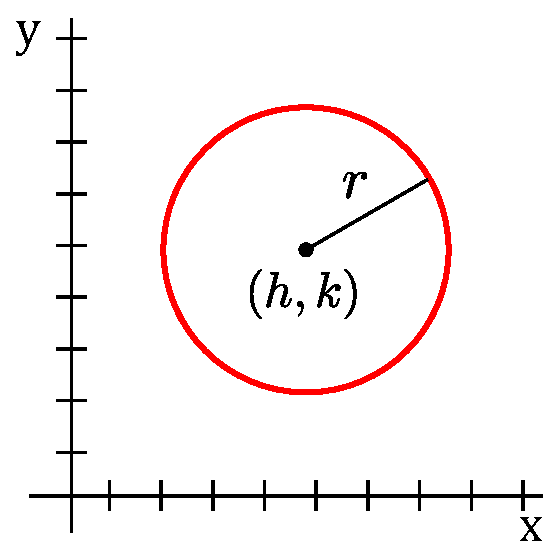
\includegraphics[width=40mm]{images/conics3}$$
\begin{multicols}{2}
\begin{itemize}
	\item $(h,k)$ is the \ifont{centre} of the circle.
	\item  $r$ is the \ifont{radius} of the circle.
\end{itemize}
\end{multicols}

\bigskip\noindent
\dfont{Ellipse:} The equation of an ellipse is:
$$\frac{(x-h)^2}{a^2}+\frac{(y-k)^2}{b^2}=1$$
$$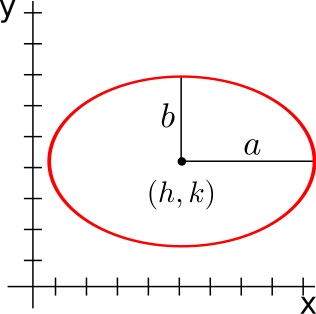
\includegraphics[width=40mm]{images/conics4}$$
\begin{itemize}
	\item $(h,k)$ is the \ifont{centre} of the ellipse.
	\item $a$ is the \ifont{horizontal distance} from the centre to the edge of the ellipse.
	\item $b$ is the \ifont{vertical distance} from the centre to the edge of the ellipse.
\end{itemize}

\bigskip\noindent
\dfont{Horizontal Hyperbola:} The equation of a horizontal hyperbola is:
$$\frac{(x-h)^2}{a^2}-\frac{(y-k)^2}{b^2}=1$$
%$$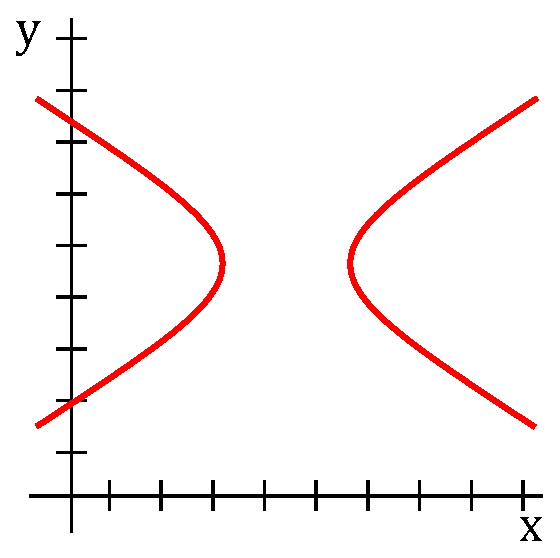
\includegraphics[width=40mm]{images/conics5}$$
\begin{multicols}{2}
\begin{itemize}
	\item $(h,k)$ is the \ifont{centre} of the hyperbola.
	\item $a,b$ are the \ifont{reference box} values. The box has a centre of $(h,k)$.
	\item $a$ is the \ifont{horizontal distance} from the centre to the edge of the box.
	\item $b$ is the \ifont{vertical  distance} from the centre to the edge of the box.
\end{itemize}
\end{multicols}
Given the equation of a horizontal hyperbola, one may sketch it by first placing a dot at 
the point $(h,k)$. Then draw a box around $(h,k)$ with horizontal distance $a$ and vertical distance $b$ to the edge of the box. Then draw dotted lines (called the \dfont{asymptotes} of the hyperbola) through the corners of the box. Finally, sketch the hyperbola in a horizontal direction as illustrated below.
$$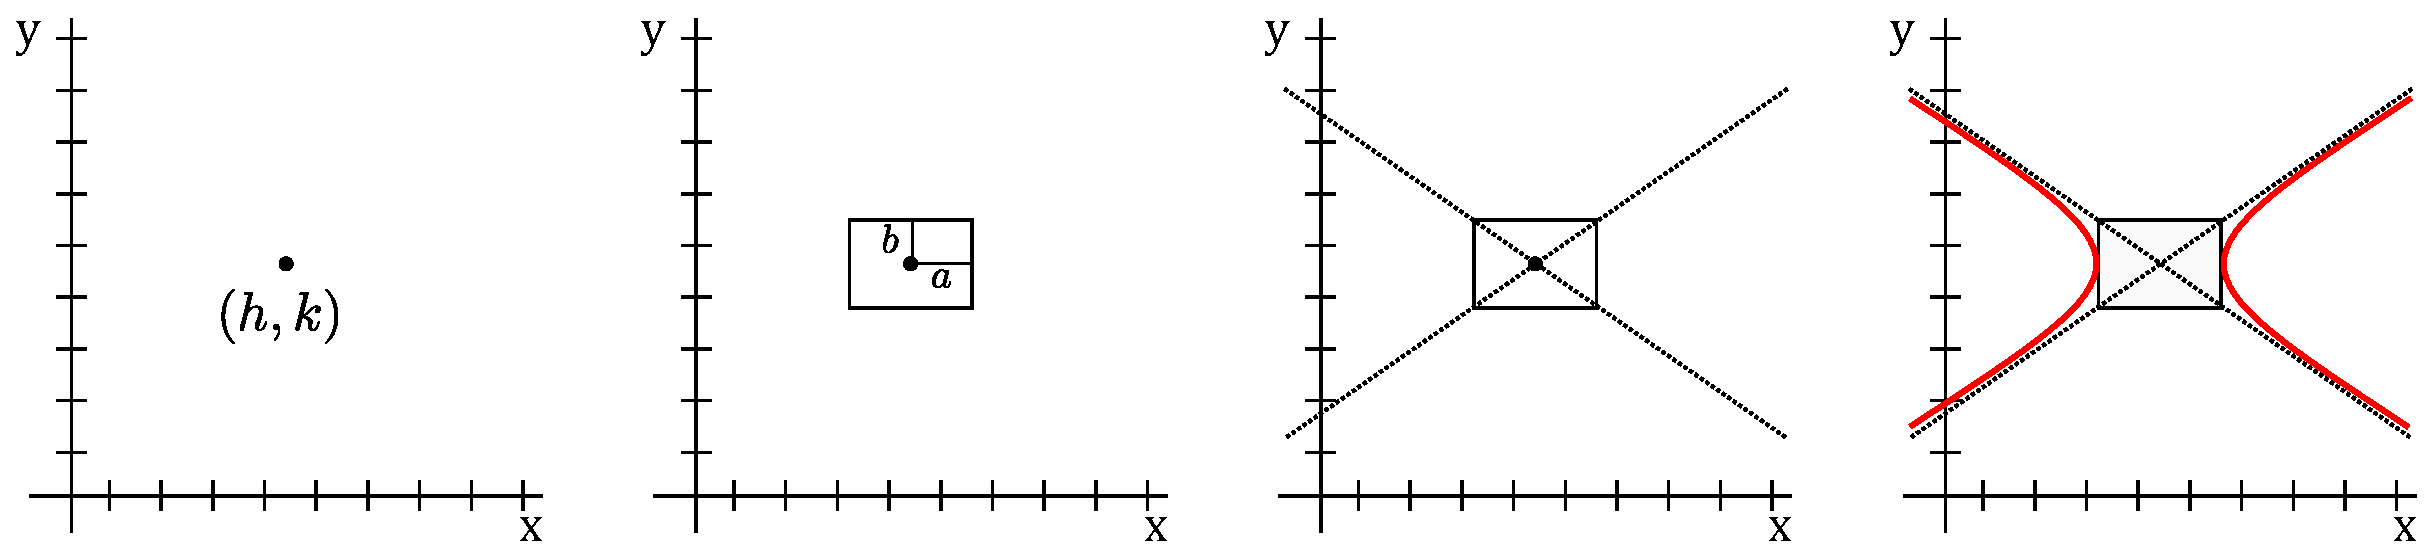
\includegraphics[width=150mm]{images/conics6}$$

\bigskip\noindent
\dfont{Vertical Hyperbola:} The equation of a vertical hyperbola is:
$$\frac{(x-h)^2}{a^2}-\frac{(y-k)^2}{b^2}=-1$$
%$$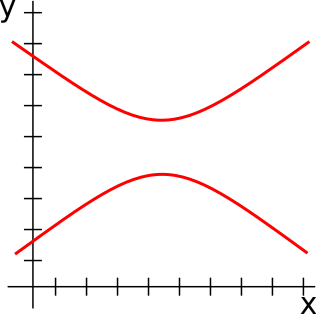
\includegraphics[width=40mm]{images/conics7}$$
\begin{multicols}{2}
\begin{itemize}
	\item $(h,k)$ is the \ifont{centre} of the hyperbola.
	\item $a,b$ are the \ifont{reference box} values. The box has a centre of $(h,k)$.
	\item $a$ is the \ifont{horizontal distance} from the centre to the edge of the box.
	\item $b$ is the \ifont{vertical  distance} from the centre to the edge of the box.
\end{itemize}
\end{multicols}
Given the equation of a vertical hyperbola, one may sketch it by following the same steps as with a horizontal hyperbola, but sketching the hyperbola going in a vertical direction.
$$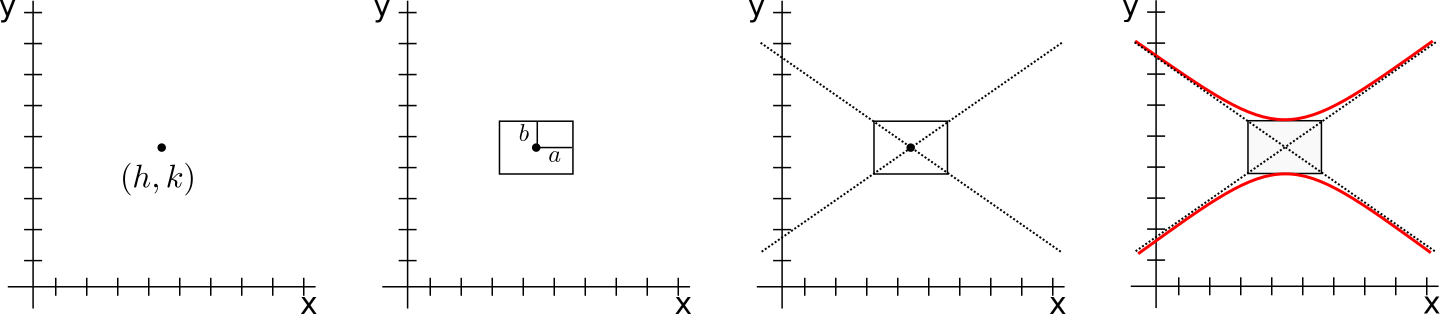
\includegraphics[width=150mm]{images/conics8}$$

\begin{formulabox}[Determining the Type of Conic]
An equation of the form
$$Ax^2+Bxy+Cy^2+Dx+Ey+F=0$$
gives rise to a graph that can be generated by performing a conic section (parabolas, circles, ellipses, hyperbolas).
Note that the $Bxy$ term involves conic rotation. The $Dx$, $Ex$, and $F$ terms affect the vertex and centre.
For simplicity, we will omit the $Bxy$ term.
To determine the type of graph we focus our analysis on the values of $A$ and $C$.
\begin{itemize}\setlength{\itemsep}{0 in}
	\item If $A=C$, the graph is a \ifont{circle}.
	\item If $AC>0$ (and $A\neq C$), the graph is an \ifont{ellipse}.
	\item If $AC=0$, the graph is a \ifont{parabola}.
	\item If $AC<0$, the graph is a \ifont{hyperbola}.
\end{itemize}
\end{formulabox}

%\subsubsection{Completing the square}
%The technique of \dfont{completing the square} allows us to determine the center of a circle/ellipse or the vertex of a parabola.
%It is also an important technique used for other purposes (for example, to derive the quadratic formula you can start by completing the square in $ax^2+bx+c=0$, $a\neq 0$).
%
%The main idea behind completing the square is to turn:
%$$ ax^2 + bx + c$$
%into
%$$a(x - h)^2 + k.$$
%One way to complete the square is to use the following formula:
%$$ax^2+bx+c=a\left(x+\frac{b}{2a}\right)^2-\frac{b^2}{4a^2}+c.$$
%But this formula is a bit complicated, so some students prefer following the steps outlined in the next example.
%
%\begin{example}{Completing the Square}{CompletingSquare}
%Solve $2x^2+12x-32=0$ by completing the square.
%\end{example}
%
%\begin{solution}
%In this instance, we will \ifont{not} divide by $2$ first (usually you would) in order to demonstrate what you should do when the `$a$' value is not $1$.
%
%\bigskip
%
%\begin{tabular}{rl}
%$2x^2+12x-32=0$ & Start with original equation.\\
%\\
%$2x^2+12x=32$ & Move the number over to the other side.\\
%\\
%$2(x^2+6x)=32$ & Factor out the $a$ from the $ax^2+bx$ expression.\\
%\\
%$6~~\to~~\frac{6}{2}=3~~\to~~3^2=\dfont{9}$ & Take the number in front of $x$, \\
%	&  \dfont{divide by $2$}, \\
%	&  then \dfont{square} it.\\
%\\
%$\ifont{2}(x^2+6x+\dfont{9})=32+\ifont{2}\cdot\dfont{9}$ & Add the result to both sides, \\
%	&  taking $a=2$ into account.\\
%\\
%$2(x+3)^2=50$ & Factor the resulting perfect square trinomial.\\
%\\
%~ & \ifont{You have now completed the square!}\\
%\\
%$(x+3)^2=25~~\to~~x=2 \mbox{ or } x=-8$ & To solve for $x$, simply divide by $a=2$ \\
%	& and take square roots.\\
%\end{tabular}
%\end{solution}

\begin{example}{Center and Radius of a Circle}{CenterRadius}
Find the centre and radius of the circle $y^2 + x^2 - 12x + 8y + 43 = 0$.
\end{example}

\begin{solution} 
We need to complete the square twice, once for the $x$ terms and once for the $y$ terms.
We'll do both at the same time.
First let's collect the terms with $x$ together, the terms with $y$ together, and move the number to the other side.
%$$y^2 + x^2 - 12x + 8y + 43 = 0$$
$$(x^2-12x)+(y^2+8y)=-43$$
We add $36$ to both sides for the $x$ term ($-12\to \frac{-12}{2}=-6\to (-6)^2=36$), and $16$ to both sides for the $y$ term ($8\to \frac{8}{2}=4\to (4)^2=16$):
$$(x^2-12x+36)+(y^2+8y+16)=-43+36+16$$
Factoring gives:
$$(x-6)^2+(y+4)^2=3^2.$$
Therefore, the centre of the circle is $(6,-4)$ and the radius is $3$.
\end{solution} 

\begin{example}{Type of Conic}{TypeConic}
What type of conic is $4x^2-y^2-8x+8=0$?
Put it in standard form.
\end{example}

\begin{solution} 
Here we have $A=4$ and $C=-1$.
Since $AC<0$, the conic is a hyperbola.
Let us complete the square for the $x$ and $y$ terms.
First let's collect the terms with $x$ together, the terms with $y$ together, and move the number to the other side.
$$(4x^2-8x)-y^2=-8$$
Now we factor out $4$ from the $x$ terms.
$$4(x^2-2x)-y^2=-8$$
Notice that we don't need to complete the square for the $y$ terms (it is already completed!). To complete the square for the $x$ terms we add \dfont{1} ($-2\to\frac{-2}{2}=-1\to(-1)^2=1$), taking into consideration that the $a$ value is $4$:
$$\ifont{4}(x^2-2x+\dfont{1})-y^2=-8+\ifont{4}\cdot\dfont{1}$$
Factoring gives:
$$4(x-1)^2-y^2=-4$$
A hyperbola in standard form has $\pm1$ on the right side and a positive $x^2$ on the left side, thus, we must divide by $4$:
$$(x-1)^2-\frac{y^2}{4}=-1$$
Now we can see that the equation represents a vertical hyperbola with centre $(1,0)$ (and with $a$ value $\sqrt{1}=1$, and $b$ value $\sqrt{4}=2$).
\end{solution} 




\begin{example}{Equation of Parabola}{EquationParabola}\label{EquationParabola}
Find an equation of the parabola with vertex $(1,-1)$ that passes through the points $(-4, 24)$ and $(7, 35)$.
\end{example}

\begin{solution} 
We first need to determine if it is a vertical parabola or horizontal parabola.
See figure \ref{fig:EquationParabola} for a sketch of the three points $(1,-1)$, $(-4, 24)$ and $(7, 35)$ in the $xy$-plane.
\figure[!ht]
$$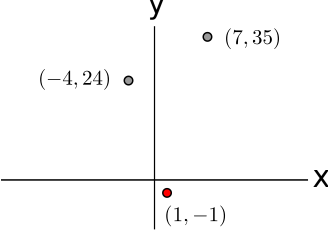
\includegraphics[width=60mm]{images/conics9}$$
\caption{Figure for Example \ref{EquationParabola}\label{fig:EquationParabola}}
\endfigure
Note that the vertex is $(1,-1)$.
Given the location of the vertex, the parabola cannot open downwards.
It also cannot open left or right (because the vertex is between the other two points - if it were to open to the right, every other point would need to be to the right of the vertex; if it were to open to the left, every other point would need to be to the left of the vertex).
Therefore, the parabola must open upwards and it is a vertical parabola.
It has an equation of
$$y-k=a(x-h)^2.$$
As the vertex is $(h,k)=(1,-1)$ we have:
$$y-(-1)=a(x-1)^2$$
To determine $a$, we substitute one of the points into the equation and solve.
Let us substitute the point $(x,y)=(-4,24)$ into the equation:
$$24-(-1)=a(-4-1)^2\quad\to\quad 25=25a\quad\to\quad a=1.$$
Therefore, the equation of the parabola is:
$$y+1=(x-1)^2.$$
Note that if we substituted $(7,35)$ into the equation instead, we would also get $a=1$.
\end{solution}


